\documentclass{beamer}
\usetheme{Copenhagen}
\usepackage[utf8]{inputenc}
\usepackage{amsmath}

\usepackage{tikz}
\usetikzlibrary{automata, positioning}

\usepackage{subfiles}

\newcommand*\dif{\mathop{}\!\mathrm{d}}

\title[Synthetic Likelihoods]{Synthetic Likelihoods for Parameter Inference in Electricity Spot Price Models}
\author{Jake Ireland}
\date{}

\begin{document}

\frame{\titlepage}

\begin{frame}{Outline}
        \begin{itemize}
            \item Part I: Features of Spot Electricity Prices and a Model
            \item Part II: What is a Synthetic Likelihood?
            \item Part III: Fitting \& Results
        \end{itemize}
\end{frame}

\begin{frame}{Part I: Features of Electricity Spot Prices}
    Features of Electricity Prices:
    \begin{itemize}
        \item Large Volatility, Mean Reversion, Seasonality, Price Spikes
    \end{itemize}
    
    \begin{figure}[H]
        \centering
        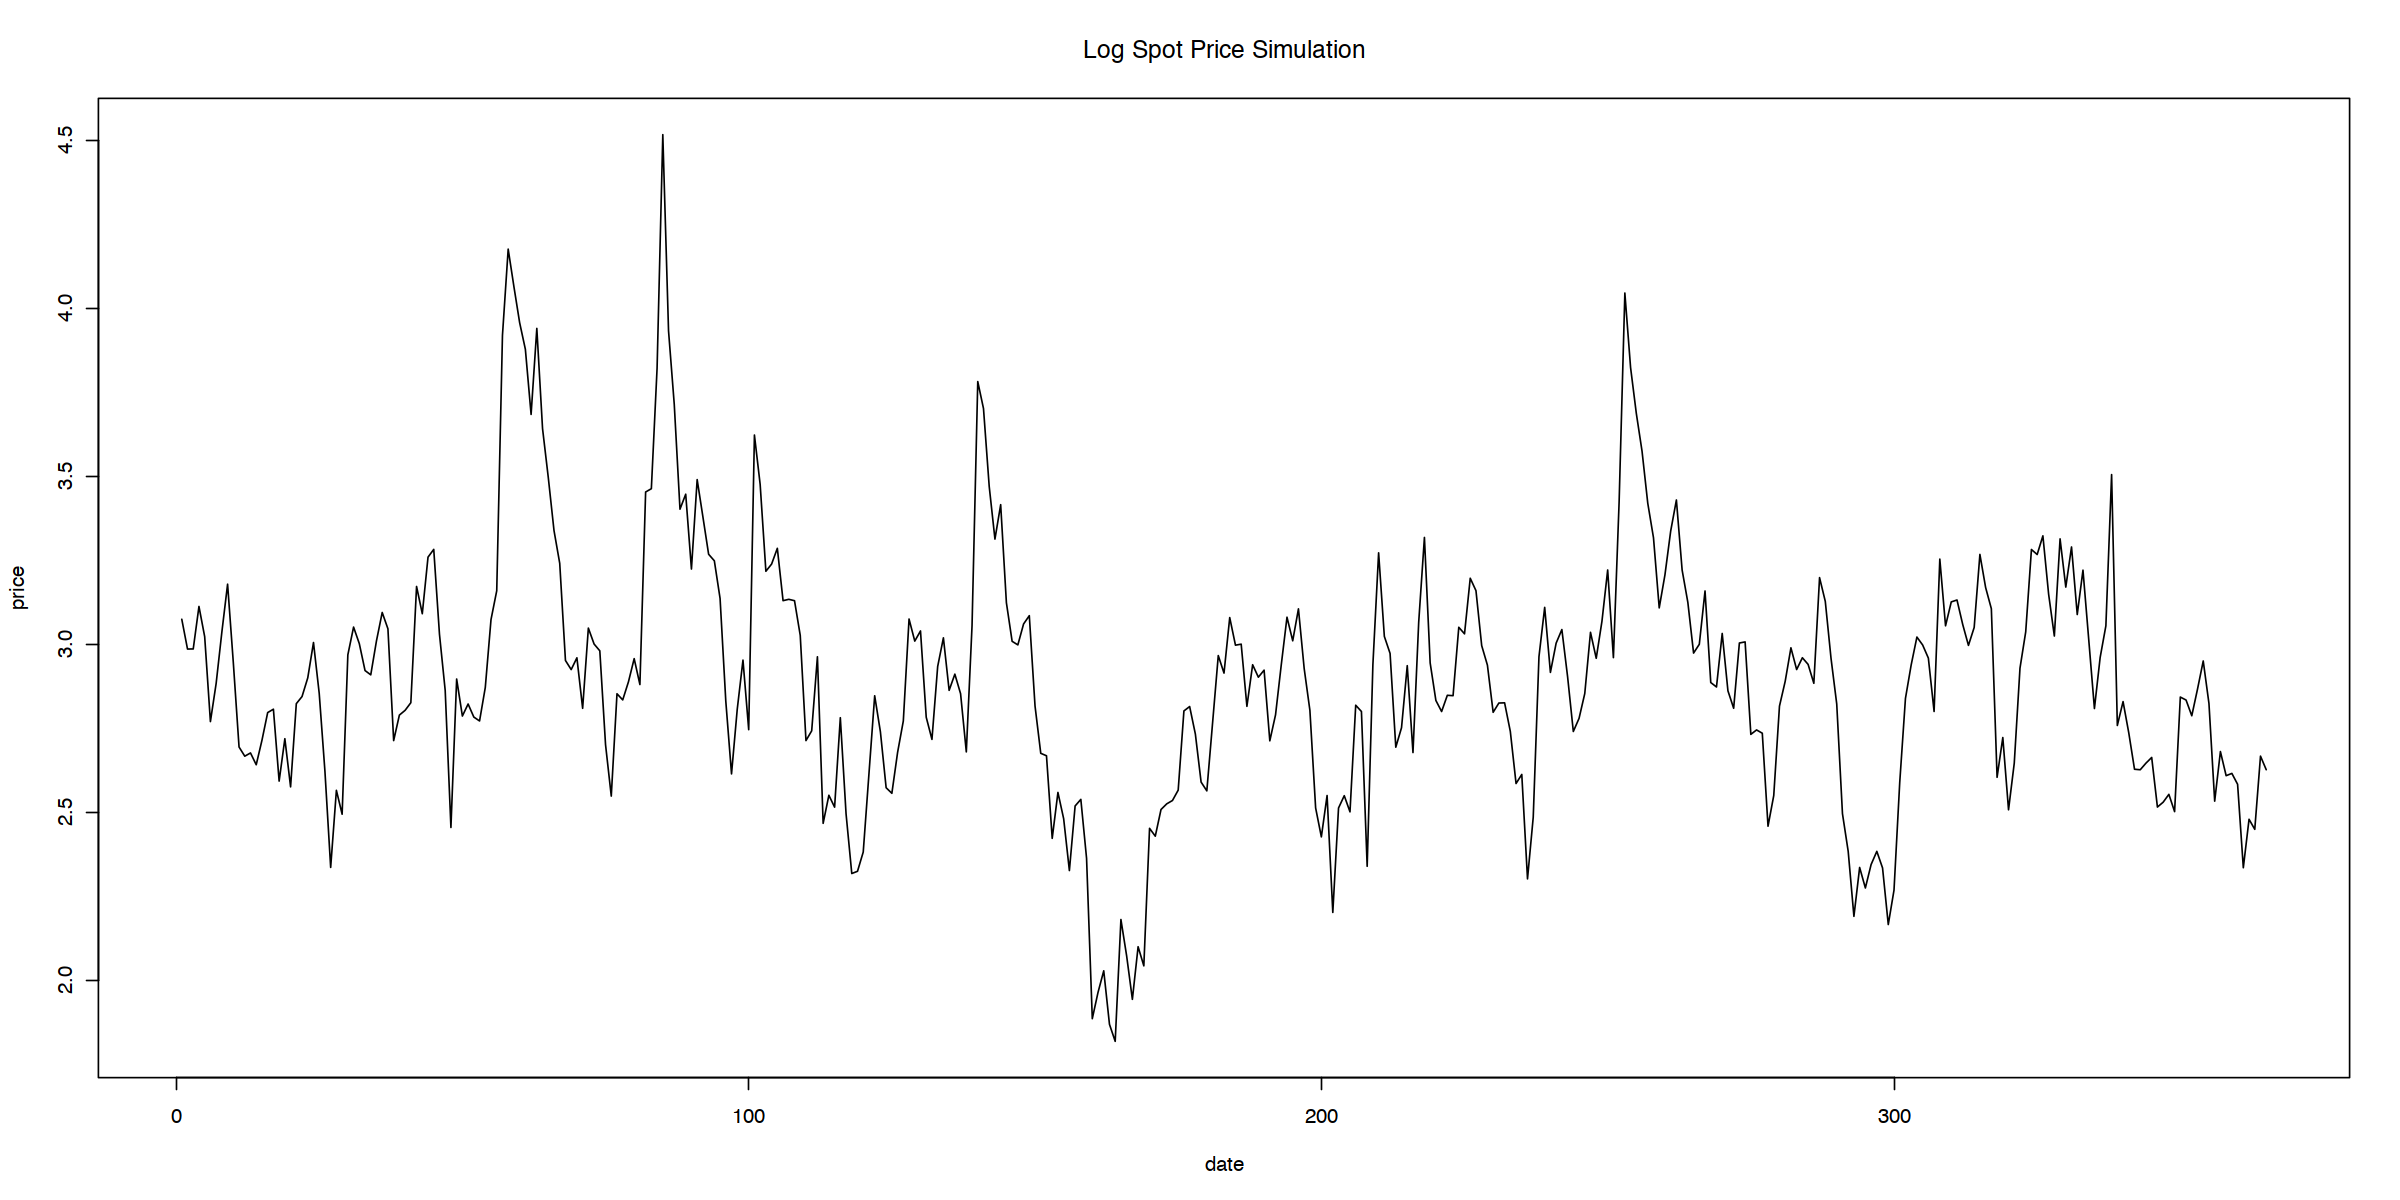
\includegraphics[width=90mm]{ex_traj.png}
        \caption{Example Trajectory from Model}
    \end{figure}
\end{frame}

\begin{frame}{Part I: Electricity Spot Price Model}
    We can account for these features by using a regime-switching model (Huisman \& Mahieu 2003). We need three regimes:
    \begin{itemize}
        \item Regime $0$: Default Price Levels.
        \item Regime $1$: A price Spike.
        \item Regime $-1$: Reverting after a price spike.
    \end{itemize}
    Switching between regimes is given by the Markov process below where $p$ is the probability of remaining in Regime $0$.
    \subfile{transitiondiagram}
    
\end{frame}

\begin{frame}{Part I: Mathematical Specification of the Model}
    Let $s(t)$ be the natural log of the spot price on day $t$. Let $(\epsilon(t))$ be a sequence of iid standard Normal random variables.
    \\
    \begin{itemize}
        \setlength\itemsep{1em}
        \item $s(t) = f(t) + x(t)$
        \item $f(t) = \mu_0 + \beta_1 D_1(t) + \beta_2 D_2(t)$
        \item $\dif x(t) := x(t) - x(t-1)$, $x(0)=0$
        \item $ \dif x(t) = \begin{cases}
        -\alpha_0 x(t-1) + \sigma_0 \epsilon(t) & \text{Day $t$ in Regime $0$} \\
        \mu_1 + \sigma_1 \epsilon(t) & \text{Day $t$ in Regime $1$} \\
        -\alpha_{-1} x(t-1) + \sigma_{-1} \epsilon(t) & \text{Day $t$ in Regime $-1$} \end{cases} $
    \end{itemize}
\end{frame}

%\begin{frame}{Part II: What is a Synthetic Likelihood?}

%\begin{itemize}
%    \item Model: $f(x|\pmb{\theta})$, Observations: $x_1, x_2, \ldots, x_N$
%    \item MLE: $\pmb{\theta}_{\text{MLE}}$ chosen as the $\pmb{\theta}$ to maximise $\sum_{i=1}^N \log{f(x_i)|\pmb{\theta})}$
%    \item Issues:
%    \begin{itemize}
%        \item Needs tractable (closed-form) $f(x|\pmb{\theta})$
%        \item Double Penalty Problem (can't approximate $f(x|\pmb{\theta})$)
%   \end{itemize}
%\end{itemize}

%\begin{figure}[H]
%    \centering
%    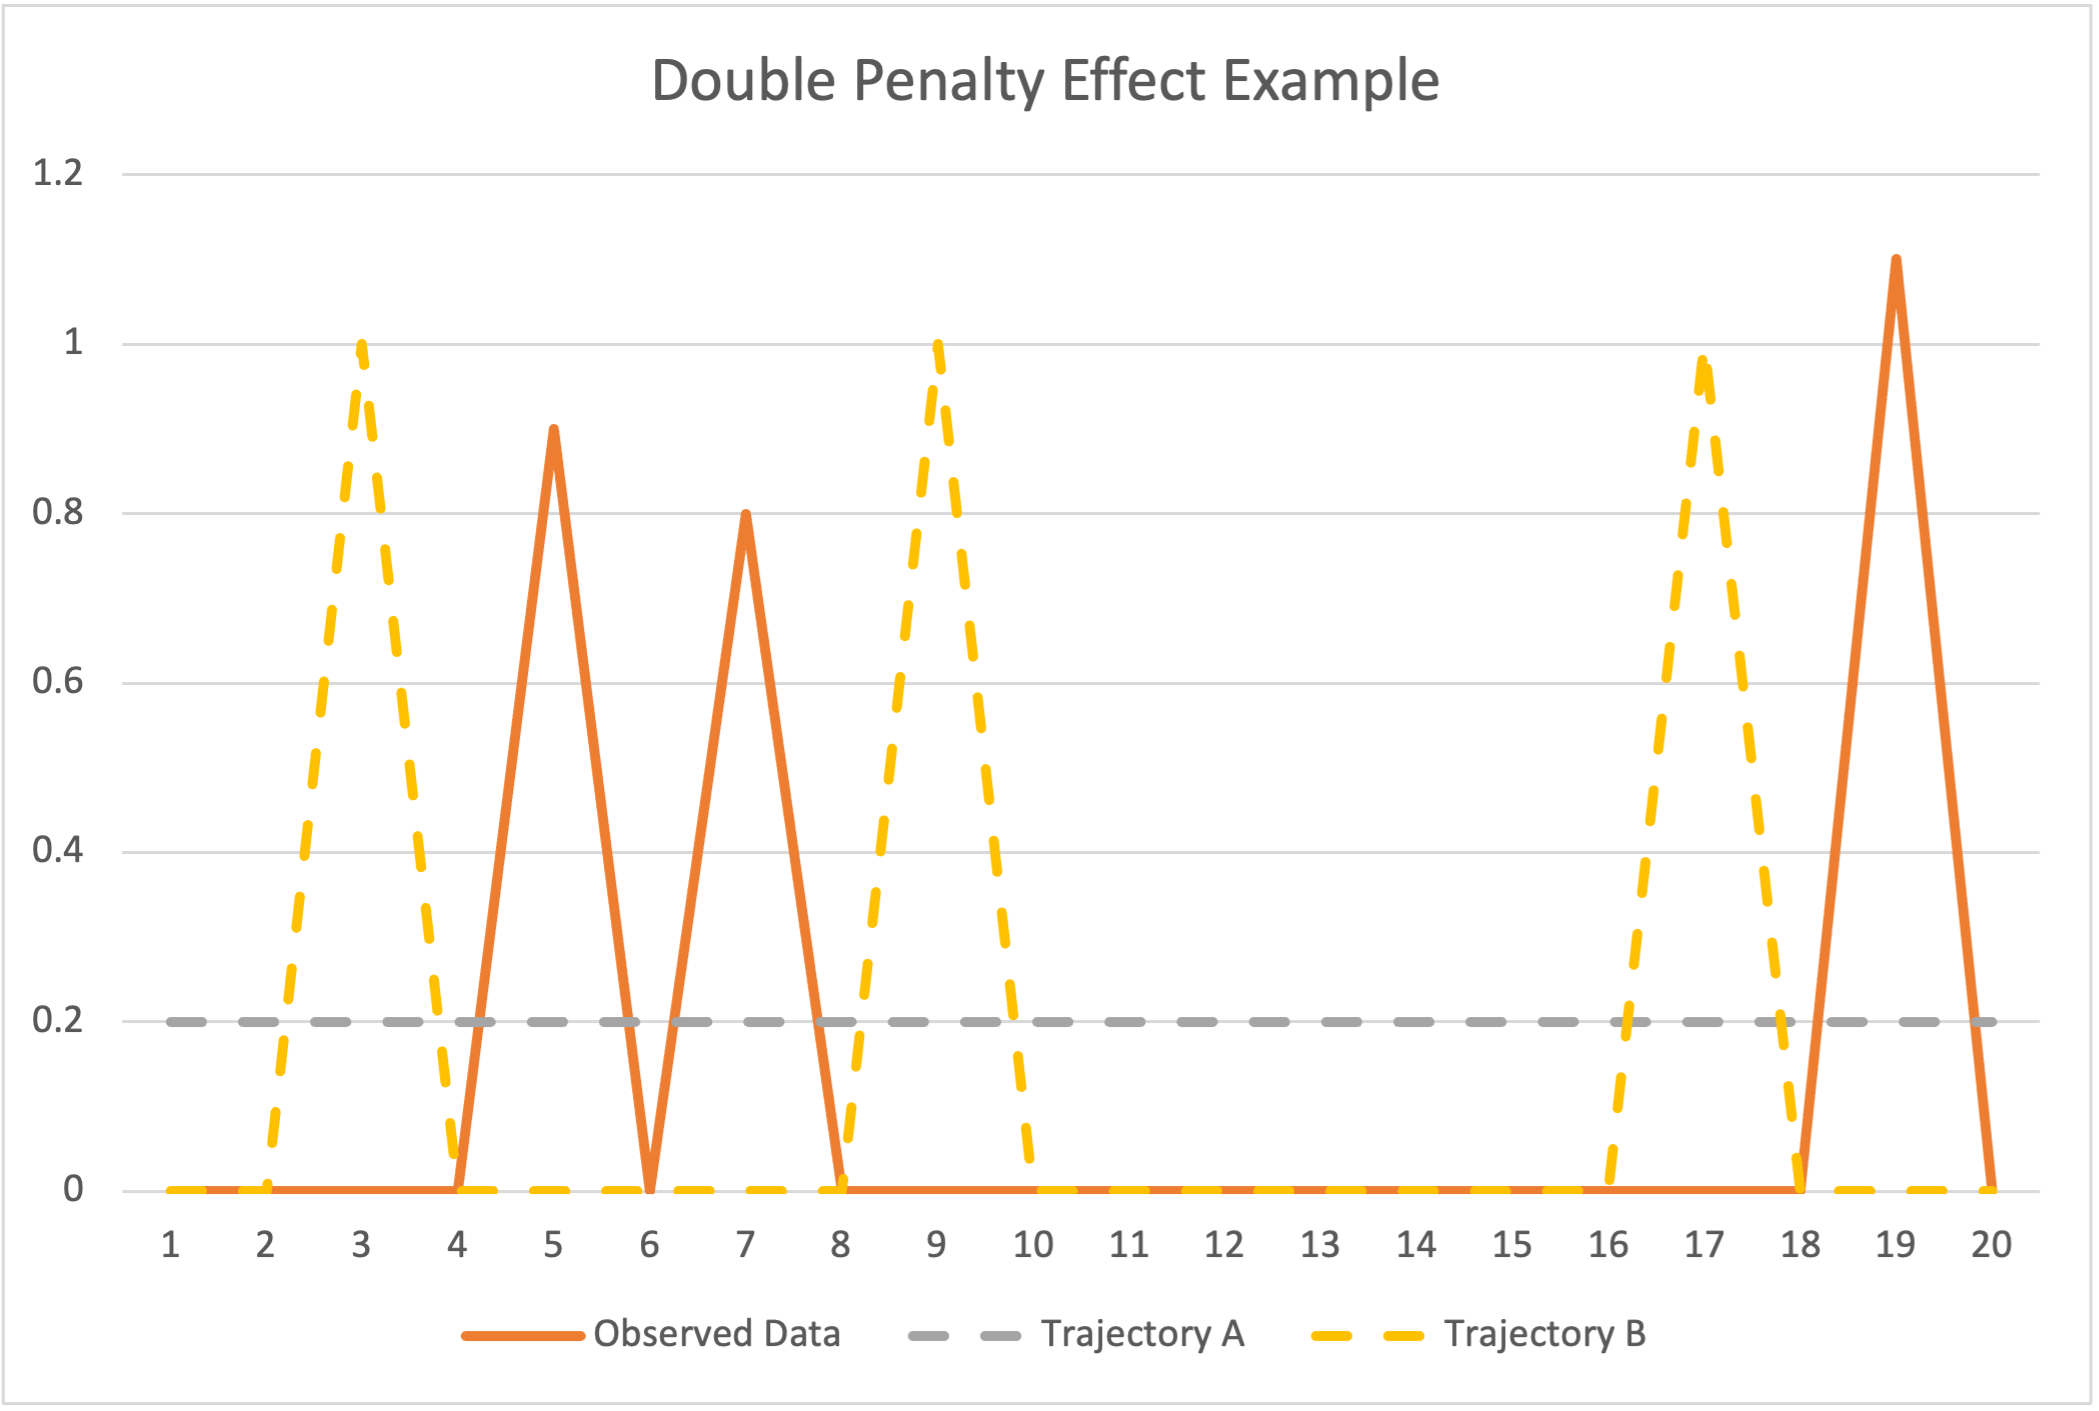
\includegraphics[width=70mm]{double_penalty_excel.png}
%    \caption{Double Penalty Effect}
%    \label{fig:double-penalty}
%\end{figure}

%\end{frame}

\begin{frame}{Part II: What is a Synthetic Likelihood?}

\begin{itemize}
    \item Model: $f(\pmb{y}|\pmb{\theta})$, Observed trajectory: $\pmb{y}_0$
    \item Idea:
    \begin{itemize}
        \item MLE: choose parameters that maximise the chance of seeing the observed trajectory 
        \item SLE: choose parameters that maximise the chance of a trajectory presenting some observed summary statistics.
    \end{itemize}
    \item Issue: Computationally intensive (and choosing good statistics)
    \item Solution: Robust Covariance Matrix
    \item Issue: Need $M$-Statistics (we can write each statistic as the minimisation of a loss function)
\end{itemize}

\end{frame}

\begin{frame}{Part II: Technical Details}

\begin{block}{Synthetic Likelihood Estimation (Wood 2010)}
    \begin{itemize}
        \item Choose statistics: $\pmb{s}(\cdot) = (s_1(\cdot), \ldots, s_M(\cdot)) \sim \mathcal{N}(\pmb{\mu}, \Sigma)$
        \item For some given parameters $\pmb{\theta}$:
        \begin{itemize}
            \item Generate samples: $\pmb{y}_1, \dots \pmb{y}_N$
            \item Transform samples to statistics: $\pmb{s}(\pmb{y}_1), \ldots, \pmb{s}(\pmb{y}_N)$
            \item Calculate sample mean $\hat{\pmb{\mu}}$ and covariance $\hat{\Sigma}$ of statistics
            \item Compute Synthetic Likelihood $\log{\phi(\pmb{s}(\pmb{y}_0) | \hat{\pmb{\mu}}, \hat{\Sigma})}$
        \end{itemize}
        \item $\pmb{\theta}_{\text{SLE}}$ chosen as the $\pmb{\theta}$ to maximise $\log{\phi(\pmb{s}(\pmb{y}_0) | \hat{\pmb{\mu}}, \hat{\Sigma})}$
    \end{itemize}
\end{block}

\begin{block}{Robust Covariance Matrix (Huber 1967)}
    \begin{itemize}
        \item Write each statistic $s_i(\cdot)$ as the minimisation of loss function $L_i$. Define $L := \sum_{i=1}^M L_i$.
        \item Compute the hessian $H_L$ of $L$ and V, the sample covariance of the gradient of $L$ (taken over each element of the trajectory).
        \item $\Sigma \approx \tilde{\Sigma} := H_L^{-1} V_{L} H_{L}^{-1}$
    \end{itemize}
\end{block}
\end{frame}

\begin{frame}{Part II: What statistics can we include?}

\begin{block}{$M$-Estimators}
    \begin{itemize}
        \item ML estimators (minimum of negative log-likelihood)
        \begin{itemize}
            \item mean, standard deviation, gamma shape parameter
        \end{itemize}
        \item Regression Coefficients (minimum of squared residuals sum)
        \begin{itemize}
            \item auto-linear regression - useful for those pesky mean-reversion parameters
            \item polynomial regression of ordered simulation values on ordered observation values
        \end{itemize}
    \end{itemize}
\end{block}

\begin{block}{Not $M$-Estimators}
    \begin{itemize}
        \item Autocorrelation coefficients
        \item mean - median
        \item quartiles (min, Q1, median, Q3, max)
        \item more complex statistics
    \end{itemize}
\end{block}
    
\end{frame}

\begin{frame}{Part II: What is a useful statistic?}

\begin{itemize}
    \item Good statistics demonstrate high correlation with model parameters and low correlation with other statistics
    \item We can conduct simulation studies to compute correlation matrices to evaluate a set of parameters
    
    \begin{figure}[H]
        \centering
        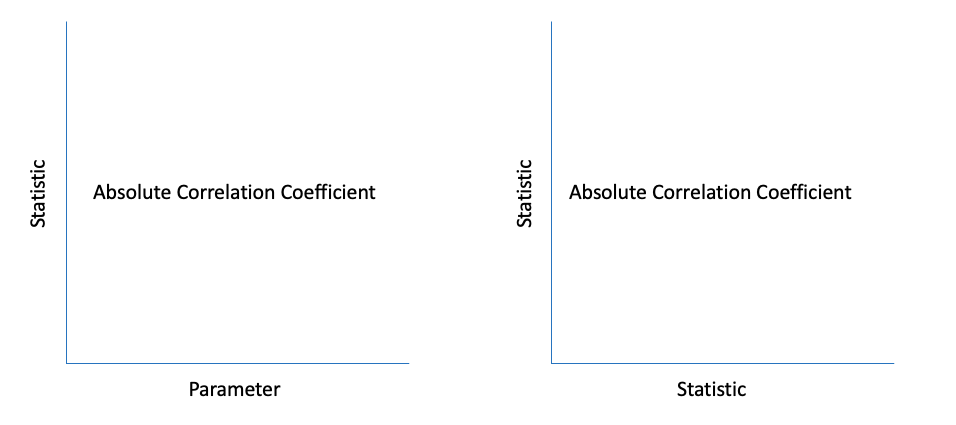
\includegraphics[width=70mm]{corr_diags.png}
        \caption{Correlation Diagrams}
    \end{figure}
\end{itemize}
    
\end{frame}

\begin{frame}{Part III: Fitting and Results}

\begin{itemize}
    \item Fitting the simplified model
    \item Computational efficiency of the RCM
    \item Full model correlation matrices
    \item Next steps
\end{itemize}
    
\end{frame}

\begin{frame}{Part III(a): Simplified Model (Set-up)}

\begin{block}{Simplified Model: Only default regime (mean reversion)}
    \begin{itemize}
        \item $s(t) = f(t) + x(t)$
        \item $f(t) = \mu_0 + \beta_1 D_1(t) + \beta_2 D_2(t)$
        \item $\dif x(t) = -\alpha_0 x(t-1) + \sigma_0 \epsilon(t)$
    \end{itemize}
\end{block}

\begin{block}{Statistics}
    \begin{itemize}
        \item We can infer $\mu_0$ and $\sigma_0$ by including the maximum likelihood estimators of normal distribution
        \item For $\beta_1$ and $\beta_2$ we can use the mean taken over Saturdays and Sundays (with a quadratic loss)
        \item For $\alpha_0$, an autoregression up to lag 1 makes sense.
        \item All $M$-Estimators!
    \end{itemize}
\end{block}



\end{frame}

\begin{frame}{Part III(a): Simplified Model (Statistics Analysis)}
    \begin{figure}
        \centering
        \subfloat{{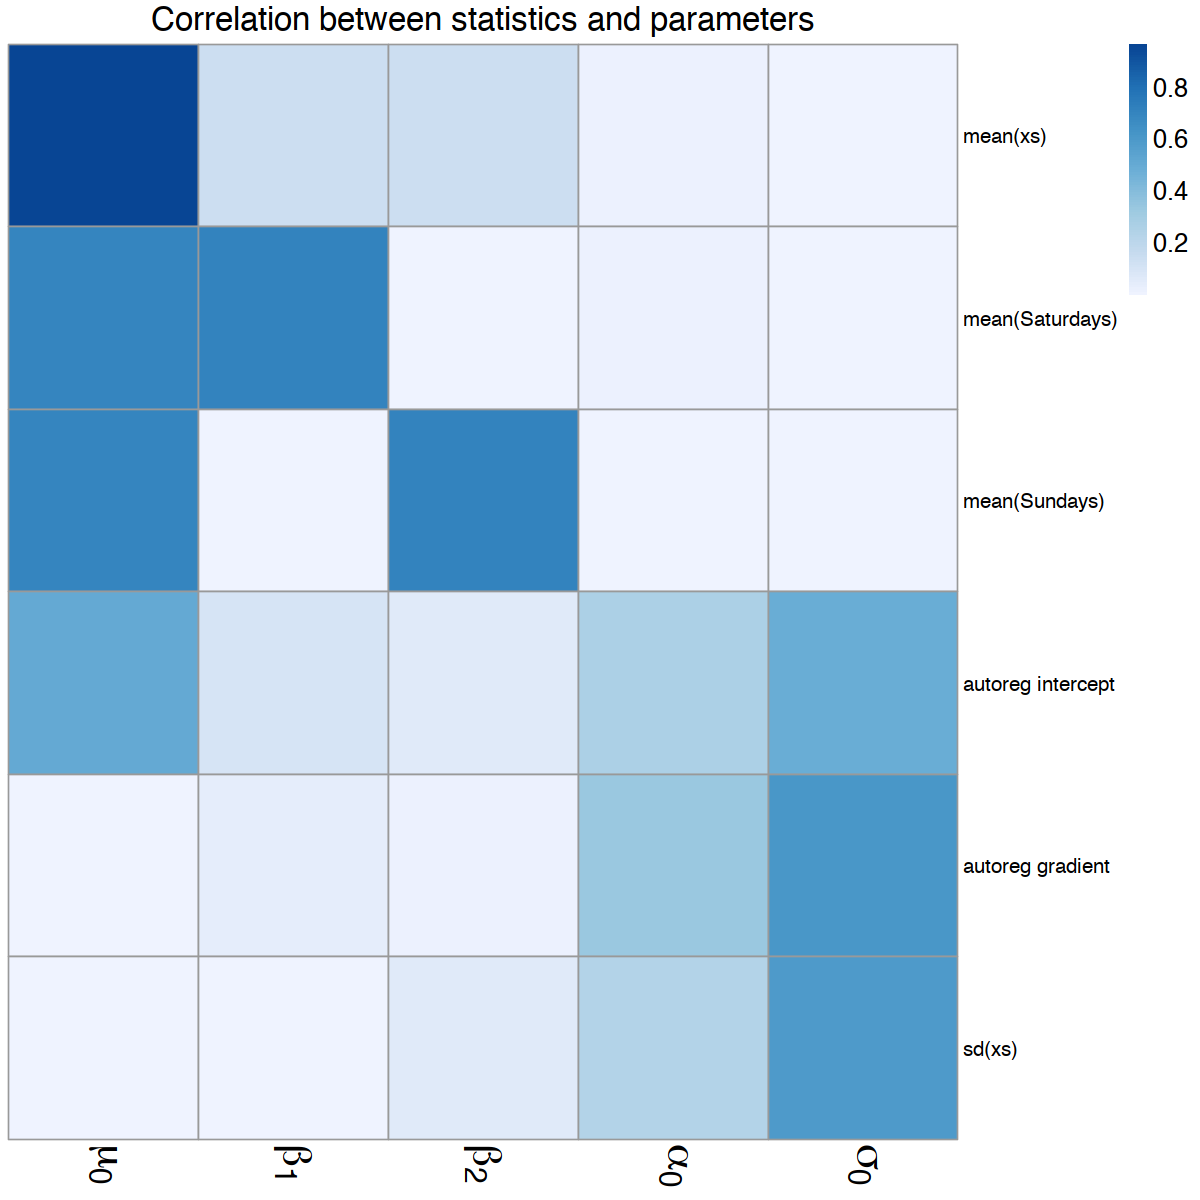
\includegraphics[width=45mm]{cor_sp.png}}}
        \qquad
        \subfloat{{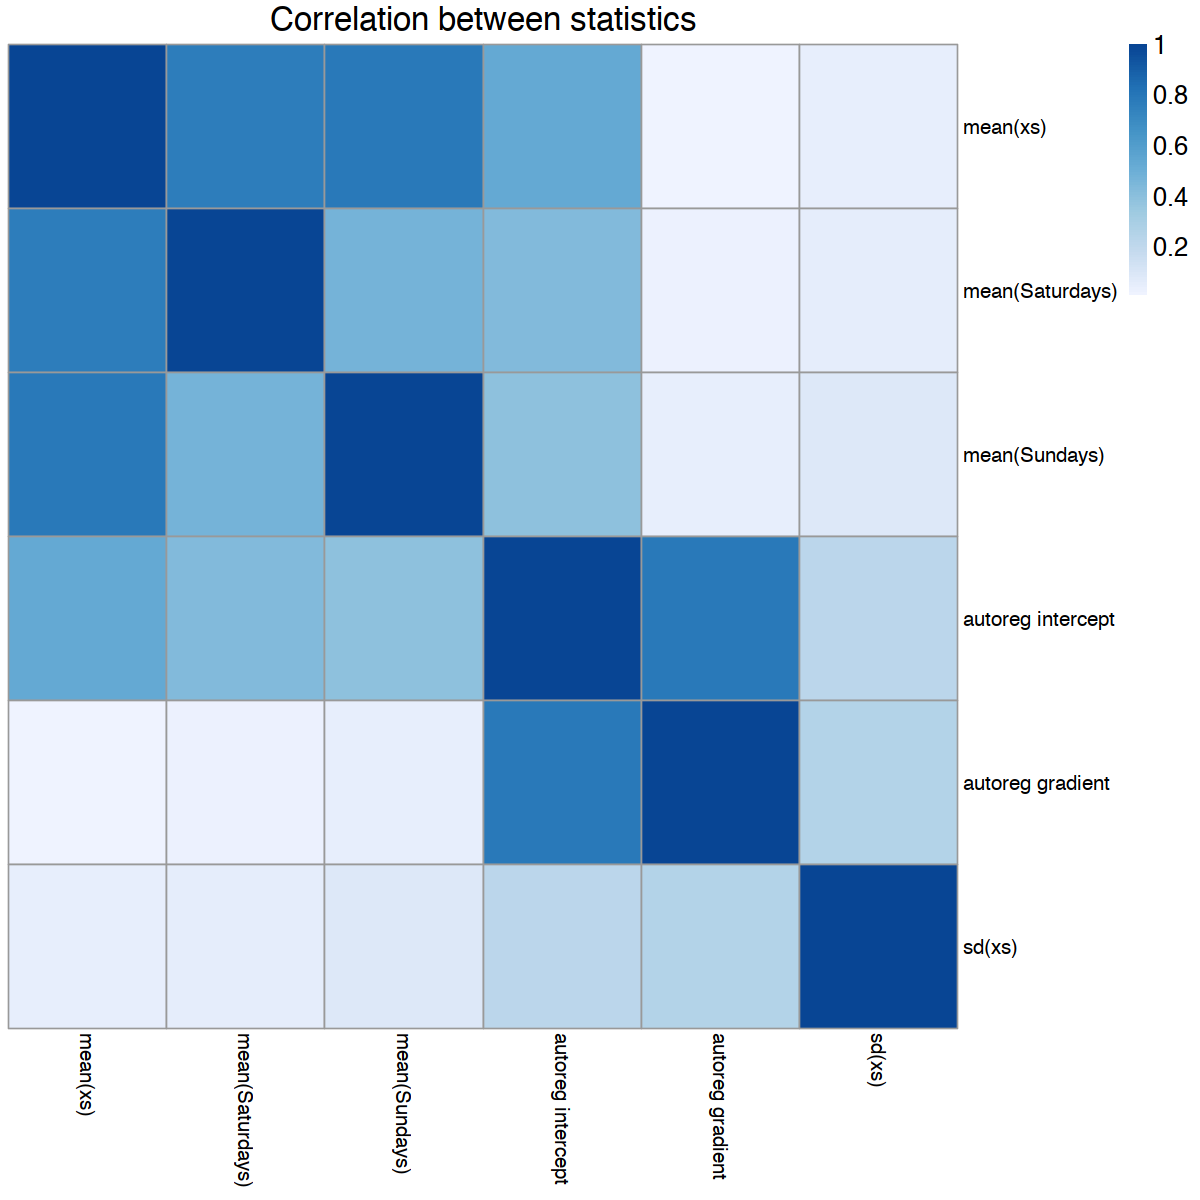
\includegraphics[width=45mm]{cor_ss.png}}}
        \caption{Correlation plots}
    \end{figure}
\end{frame}

\begin{frame}{Part III(a): Simplified Model (Simulation Study)}
    \begin{figure}[H]
        \centering
        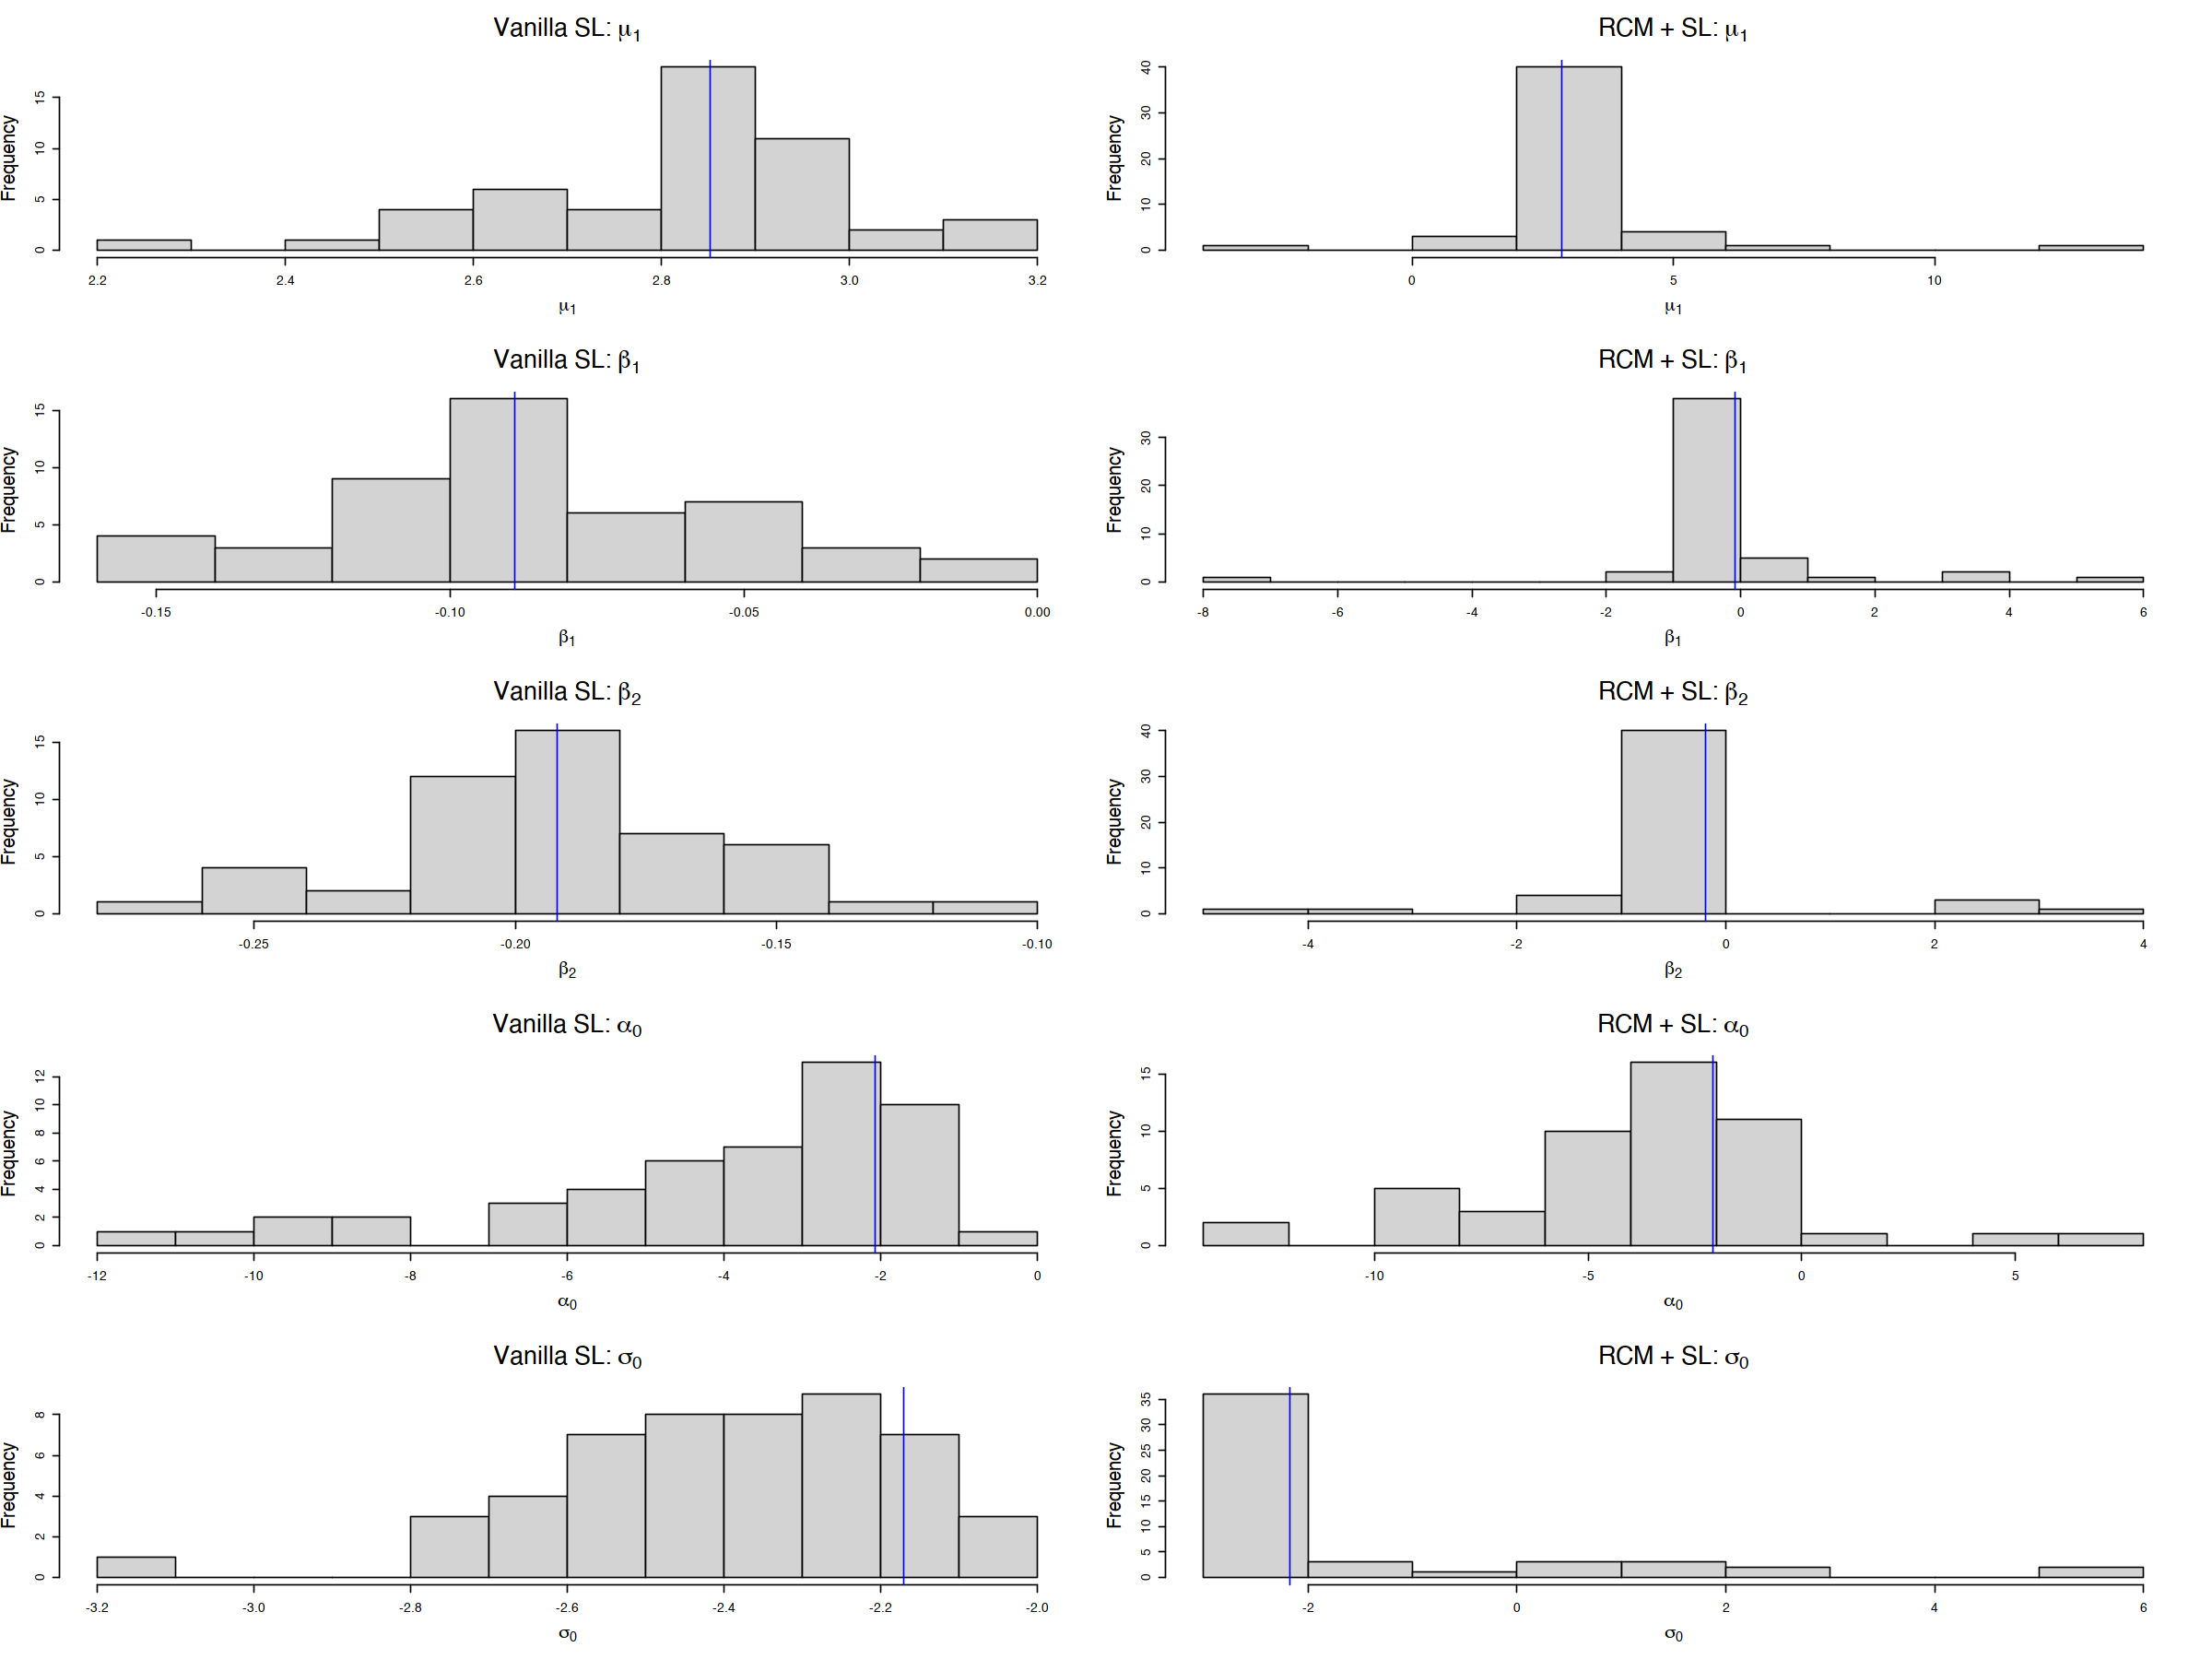
\includegraphics[width=90mm]{sim_study.png}
        \caption{Simple Model Simulation Study}
    \end{figure}
\end{frame}

\begin{frame}{Part III(b): Computational Efficiency of RCM}
    \begin{itemize}
        \item Used the \textbf{profvis} R library
        \item Wrote functions that:
        \begin{itemize}
            \item generated an `observed trajectory' using the true parameters
            \item evaluated the observed statistics
            \item calculated the synthetic likelihood of the true parameters
        \end{itemize}
        \item Evaluated the above 1000 times each
    \end{itemize}
    
    \begin{figure}
        \centering
        \subfloat{{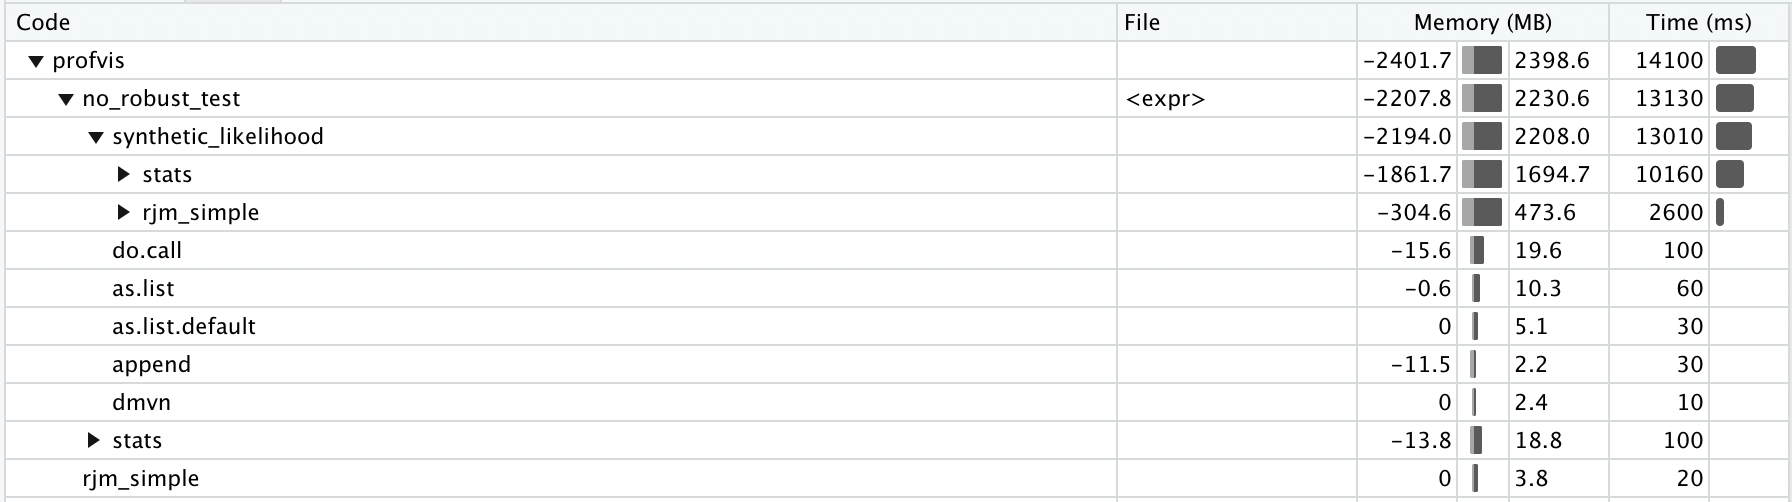
\includegraphics[width=48mm]{pv_no_robust.png}}}
        \qquad
        \subfloat{{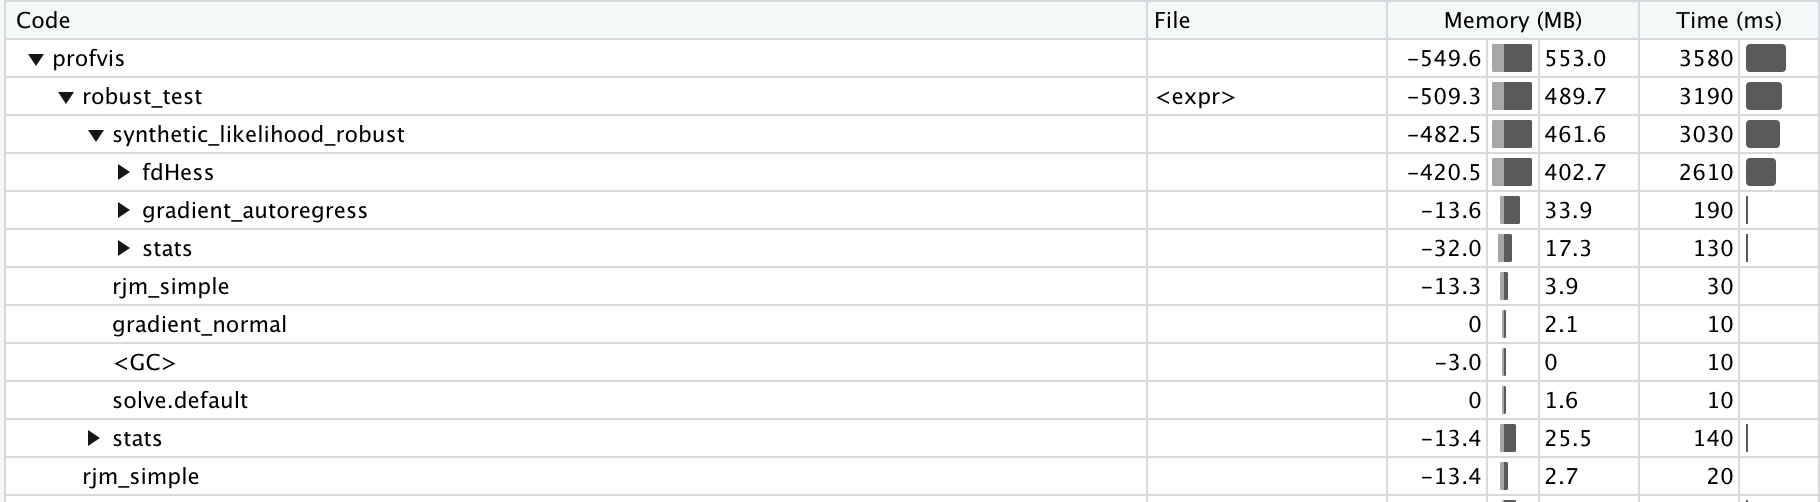
\includegraphics[width=48mm]{pv_robust.png}}}
        \caption{\textbf{profvis} results}
    \end{figure}
    
    \begin{itemize}
        \item RCM is $\approx 4 \times$ faster.
        \item Comes from needing $100 \times$ fewer samples (observation length kept the same)
    \end{itemize}
\end{frame}

\begin{frame}{Part III(c): Full model correlation matrices}
    \begin{figure}
        \centering
        \subfloat{{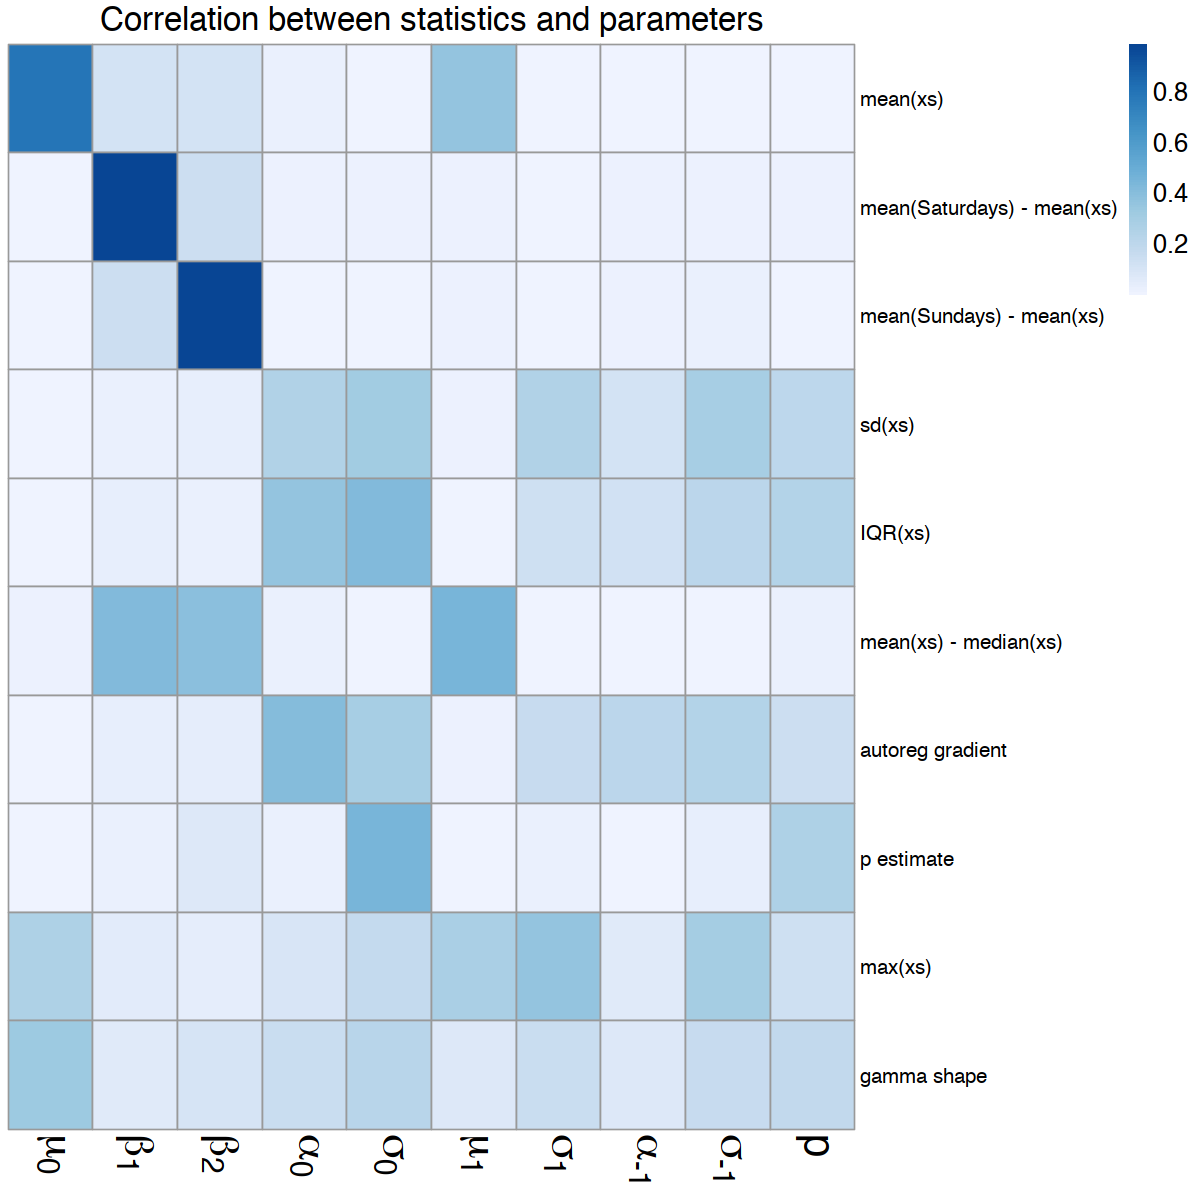
\includegraphics[width=45mm]{cor_sp_full.png}}}
        \qquad
        \subfloat{{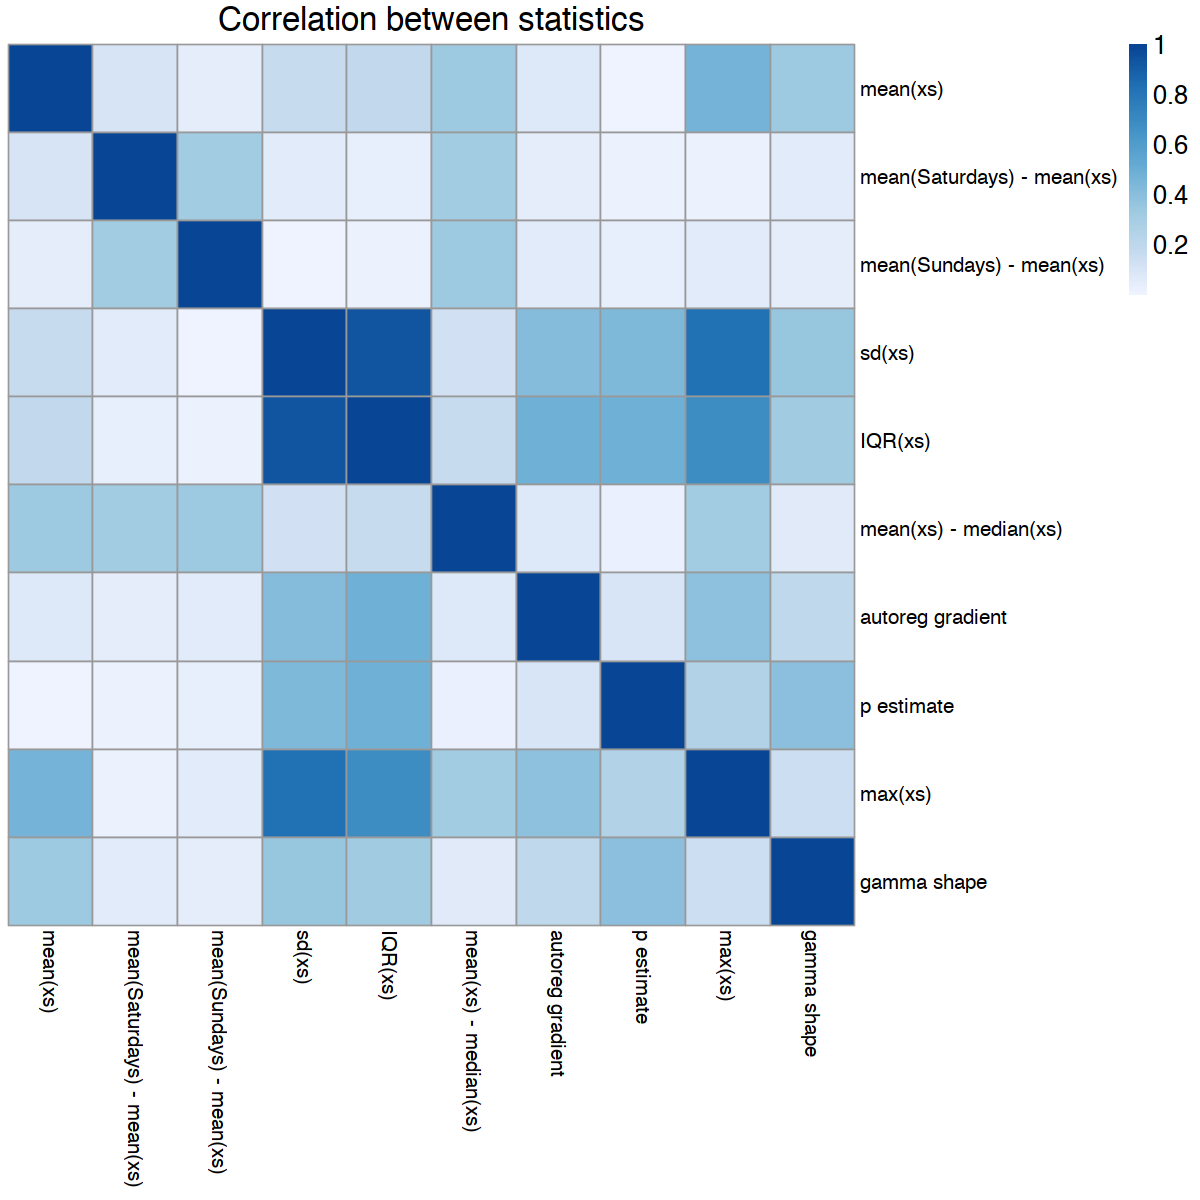
\includegraphics[width=45mm]{cor_ss_full.png}}}
        \caption{Correlation plots}
    \end{figure}
\end{frame}


\begin{frame}{Next Steps \& References}
\begin{block}{Next Steps}
    \begin{itemize}
    \item Finish fitting the full model
    \item See if non $M$-estimators can be replaced with $M$-estimators
    \item Fit actual data, use this to price financial options
\end{itemize}
\end{block}

\begin{block}{References}
    \begin{itemize}
        \item Huisman, R. and Mahieu, R., 2003. Regime jumps in electricity prices. Energy Economics, 25(5), pp.425-434.
        \item Wood, S., 2010. Statistical inference for noisy nonlinear ecological dynamic systems. Nature, 466(7310), pp.1102-1104.
        \item Huber, P., 1967. The behavior of maximum likelihood estimates under nonstandard conditions. Proceedings of the 5th Berkeley symposium on mathematical statistics and probability, 1, pp.221-233.
    \end{itemize}
\end{block}

\end{frame}

\end{document}
